\chapter{Vassiliev invariants and chord diagrams}
\label{ch:vassiliev-invariants-and-chord-diagrams}

\lettrine{\libertineInitialGlyph{V}}{assiliev} invariants are sophisticated to define in terms of the space of knots from the introduction, but the axiomatic definition of Birman-Lin \cite{knot-polynomials-and-vassilievs-invariants} is much simpler. The definition also illustrates an analogy first made by Bar-Natan \cite{on-the-vassiliev-knot-invariants} in which Vassiliev invariants are ``polynomial invariants''. This is not meant in the sense that Vassiliev invariants take values in a polynomial ring (like say, the Jones polynomial), but rather that Vassiliev invariants have special properties not shared by all invariants, just as polynomial functions have special properties not shared by all functions.

\section{Singular Knots}
\label{sec:singular-knots}

\begin{definition}
	A \textbf{singular knot} is an immersion of \(S^{1}\) into \(\R^{3}\) which fails to be an embedding at finitely many singularities, and where the singularities are double-points and transverse. When a singular knot has \(m\) such singularities, we call it \textbf{\(m\)-singular}.
\end{definition}

\begin{remark}
	\label{rem:other-singularities}
	Immersions with other types of singularities, are excluded from this definition, so the word ``singular'' in ``singular knot'' refers specifically to double point singularities. In particular immersions with
	\begin{enumerate}
		\item triple points
		\item points with vanishing derivative
	\end{enumerate}
	are excluded from the definition.
\end{remark}

A singular knot with one double point is very close to two other knots, one where it's replaced by a positive crossing and one by a negative. If the conditions are right, we can extend a knot invariant to an invariant of singular knots by ``taking its derivative''.

\begin{definition}
	\label{def:derivative}
	The \textbf{derivative} \(\delta\) of a differentiable \(m\)-singular knot invariant \(f\) is
	\[\delta f \left( \double \right) = f \left( \poscross \right) - f\left( \negcross \right).\]
\end{definition}

What are the conditions? For this to be a well-defined operation, it mustn't matter which double point we choose.

\begin{definition}
	\label{def:differentiable-invariant}
	An invariant \(f\) of \(m\)-singular knots is \textbf{differentiable} if
	\begin{equation}
		\label{eq:diff}
		\tag{\diff}
		f \left( \poscross \ \double \right) - f\left( \negcross \ \double \right) = f \left( \double \ \poscross \right) - f\left( \double \ \negcross \right).
	\end{equation}
\end{definition}

If an invariant of \(m\)-singular knots is differentiable, so is its derivative, so it can be extended to any number of double points.

Rather than thinking about functions on knots satisfying certain relations, the modern version of this subject takes the philosophy of imposing relations on the objects directly.

\begin{definition}
	\label{def:differentiable-knot}
	Define \(\mathcal{K}_{m} = \operatorname{span}(\{m\text{-singular knots}\})\) modulo the following boundary relation (also known as a codifferentiability relation):
	\begin{equation}
		\label{eq:boundary}
		\tag{\diffdual}
		\poscross \ \double - \negcross \ \double = \double \ \poscross - \double \ \negcross.
	\end{equation}

	From now on, we will refer to elements \(\mathcal{K}_{m}\) as \(m\)\textbf{-singular knots}, i.e. the \ref{eq:boundary} relation will be implicit in everything.
	% TODO: Make equation reference change font to \ttfamily
\end{definition}

\begin{definition}
	\label{def:boundary}
	The \textbf{boundary} operation is the map \(\partial : \mathcal{K}_{m} \to \mathcal{K}_{m - 1}\) defined by
	\[ \double \longmapsto \poscross - \negcross .\]
\end{definition}

\begin{remark}
	The derivative operation and the \ref{eq:diff} relation are dual to the boundary operation and the \ref{eq:boundary} relation. For example, a differentiable invariant of knots is the same as a invariant of knots in \(\mathcal{K}_{m}\).
\end{remark}

Any knot invariant, \(f\) can be extended to an invariant \(f^{(m)}\) of \(m\)-singular knots by the Vassiliev skein relation
\[f^{(0)} = f\]
and
\[f^{(m + 1)}\left(\double\right) = f^{(m)}\left(\poscross\right) - f^{(m)}\left(\negcross\right).\]
Often, we omit the superscript and write
\[f\left(\double\right) = f\left(\poscross\right) - f\left(\negcross\right).\]

The Vassiliev skein relation extends a knot via its derivative, or chooses a value on \((m + 1)\)-singular knots to agree with the difference of values on its boundary.

% TODO: Could move later, even.
\begin{definitions}
	\begin{enumerate}
		\item A knot invariant \(V\) is a \textbf{Vassiliev invariant} of order (or type) \(m\) if when extended to singular knots via the Vassiliev skein relation, there is an integer \(m\) such that
		\[V\biggl( \underbrace{\double \cdots \double}_{{\scriptscriptstyle m + 1}} \biggr) = 0.\]
	\item The \textbf{order} of a Vassiliev invariant \(V\) it the highest \(m\) such that \(V\) is a Vassiliev invariant of order \(m\). (That is, the order of a Vassiliev invariant is the highest number of double points a knot \(K\) can have without \(V(K)\) having to vanish).
	\end{enumerate}
\end{definitions}

\begin{remark}
	Vassiliev invariants of order \(m\) are those that vanish after \(m + 1\) derivatives, just like degree \(m\) polynomials.
\end{remark}

\section{Integration Theory}
\label{sec:integration-theory}

To help see the bird's eye view, and following \cite{integration-of-singular-braid-invariants}, we phrase this in terms of an integration theory.

\begin{definition}
	An \textbf{integration theory} \((\mathcal{O}_{\star}, \partial_{\star})\) is a sequence
	% https://q.uiver.app/#q=WzAsNixbMSwwLCJcXG1hdGhjYWx7T31fe219Il0sWzAsMCwiXFxjZG90cyJdLFsyLDAsIlxcbWF0aGNhbHtPfV97bSAtIDF9Il0sWzMsMCwiXFxjZG90cyJdLFs0LDAsIlxcbWF0aGNhbHtPfV97MX0iXSxbNSwwLCJcXG1hdGhjYWx7T31fezB9Il0sWzEsMCwiXFxwYXJ0aWFsIl0sWzAsMiwiXFxwYXJ0aWFsIl0sWzIsMywiXFxwYXJ0aWFsIl0sWzMsNCwiXFxwYXJ0aWFsIl0sWzQsNSwiXFxwYXJ0aWFsIl1d
	\[\begin{tikzcd}
		\cdots & {\mathcal{O}_{m}} & {\mathcal{O}_{m - 1}} & \cdots & {\mathcal{O}_{1}} & {\mathcal{O}_{0}}
		\arrow["\partial", from=1-1, to=1-2]
		\arrow["\partial", from=1-2, to=1-3]
		\arrow["\partial", from=1-3, to=1-4]
		\arrow["\partial", from=1-4, to=1-5]
		\arrow["\partial", from=1-5, to=1-6]
	\end{tikzcd}\]
	of abelian groups. In case we need to refer to a specific map, \(\partial_{m}\) denote the map \(\partial\) whose domain is \(\mathcal{O}_{m}\). Note that we do not assume \(\partial^{2} = 0\).
\end{definition}

The group is \(\mathcal{O}_{0}\) is typically free abelian, and in our case is the primary object we want to study. The groups \(\mathcal{O}_{m}\) are also typically free abelian groups, and can often be thought of as \(m\)-singular objects of some kind. The map \(\partial\) takes an \(m\)-singular object \(x\) to some combination of \((m - 1)\)-singular objects near \(x\).

By fixing an abelian group \(G\) and setting \(\mathcal{O}_{m}^{\ast} = \operatorname{Hom}(\mathcal{O}_{m}, G)\), we get the sequence
% https://q.uiver.app/#q=WzAsNixbMSwwLCJcXG1hdGhjYWx7T31fe219XntcXGFzdH0iXSxbMCwwLCJcXGNkb3RzIl0sWzIsMCwiXFxtYXRoY2Fse099X3ttIC0gMX1ee1xcYXN0fSJdLFszLDAsIlxcY2RvdHMiXSxbNCwwLCJcXG1hdGhjYWx7T31fezF9XntcXGFzdH0iXSxbNSwwLCJcXG1hdGhjYWx7T31fezB9XntcXGFzdH0iXSxbMCwxLCJcXGRlbHRhIiwyXSxbMiwwLCJcXGRlbHRhIiwyXSxbMywyLCJcXGRlbHRhIiwyXSxbNCwzLCJcXGRlbHRhIiwyXSxbNSw0LCJcXGRlbHRhIiwyXV0=
\[\begin{tikzcd}
	\cdots & {\mathcal{O}_{m}^{\ast}} & {\mathcal{O}_{m - 1}^{\ast}} & \cdots & {\mathcal{O}_{1}^{\ast}} & {\mathcal{O}_{0}^{\ast}}
	\arrow["\delta"', from=1-2, to=1-1]
	\arrow["\delta"', from=1-3, to=1-2]
	\arrow["\delta"', from=1-4, to=1-3]
	\arrow["\delta"', from=1-5, to=1-4]
	\arrow["\delta"', from=1-6, to=1-5]
\end{tikzcd}\]
where \(\delta_{m}\) is the transpose of \(\partial_{m}\). The maps \(\delta\) behaves like derivatives: \(\delta(f)\) for \(f \in \mathcal{O}_{m}^{\ast}\) defines \(f\) on \(\mathcal{O}_{m + 1}^{\ast}\) as some combination of its values on ``close'' \(m\)-singular objects.

We wish to understand how to invert this process, namely:
\begin{questions}
	\label{qu:integration-theory}
	\begin{enumerate}
		\item When does a functional in \(\mathcal{O}^{\ast}_{m}\) ``integrate'' into a functional in \(\mathcal{O}^{\ast}_{m - 1}\)?
		\item Is the integral of a functional in \(\mathcal{O}_{m}^{\ast}\) uniquely defined, or are there choices to be made?
		\item When does such a functional integrate multiple times, in-particular when does it integrate \(m\) times into a functional in \(\mathcal{O}^{\ast}_{0}\), (i.e. a function on the non-singular objects)?
		\item If there are choices to be made in integration, do they affect whether the new functional is integrable again?
		\item Which functions on the non-singular objects \(\mathcal{O}_{0}\) are obtained by \(m\) consecutive integrations of functionals in \(\mathcal{O}_{m}^{\ast}\)?
	\end{enumerate}
\end{questions}
The following modules provide the tautological answers to the above questions in the general theory.
\begin{definitions}
	\label{def:integration-theory-modules}
	\begin{enumerate}
		\item The \textbf{primary obstructions to integration} are the module
			\[P\mathcal{O}_{m} = \ker{\partial_{m}}.\]
		\item The \textbf{constants of integration} are the module
			\[C\mathcal{O}_{m} = \mathcal{O}_{m} / \partial \mathcal{O}_{m + 1}.\]
		\item The \textbf{secondary obstructions to integration} are the module
			\[S\mathcal{O}_{m} = \ker{(\partial_{m + 1}\partial_{m})} / P\mathcal{O}_{m},\]
			and likewise the \textbf{order \(k\) obstructions to integration} are defined analagously.
		\item The \textbf{weights of integration} are the module
			\[W\mathcal{O}_{m} = C\mathcal{O}_{m} / \pi(P\mathcal{O}_{m})\]
			where \(\pi: \mathcal{O}_{m} \to C\mathcal{O}_{m}\) is the projection.
		\item The \textbf{finite type invariants} of order \(m\) are the module
			\[FT\mathcal{O}_{m} = \ker \delta^{m + 1},\]
			where \(\delta^{m + 1}\) denotes \(m + 1\) applications of \(\delta\) with appropriate indices, ending with \(\delta_{m}\).

	\end{enumerate}
\end{definitions}
It may not be entirely obvious how these definitons provide answers to the questions above. In the rest of this section we will see the truth of this in the case \(\mathcal{O}^{\star} = \mathcal{K}^{\star}\) which should provide good intuition for the general case.

Recall from the picture from the introduction that \(m\)-singular knots are components of the stratification of the space of knots of codimension \(m\).

\begin{definition}
	A \textbf{singular isotopy}, \(\Psi(t)\) of \(m\)-singular knots is a path in the union of the \(m\)th and \((m + 1)\)st strata such that the path only intersects the \((m + 1)\)st stratum transversally and finitely many times. The intersections \(\{\Psi_{s} : 1 \leq s \leq r\}\) of the path with the \((m + 1)\)st stratum are called the \textbf{singularities} of the singular isotopy. The \textbf{signs} \(\varepsilon_{s} = \varepsilon(s): \{s\} \to \{\pm 1\}\) of the singularities give the signs of the corresponding intersection.
\end{definition}

% TODO: Insert an image of a singular isotopy.

To rephrase the definitions in section \ref{sec:singular-knots}, in the integration theory \(\mathcal{O}^{\star} = \mathcal{K}^{\star}\), differentiation constructs from an invariant \(Q\) of \(m\)-singular knots, an invariant \(Q'\) of \((m + 1)\)-singular knots such that along singular isotopies from \(k_{0}\) to \(k_{1}\),
\[Q(k_{0}) - Q(k_{1}) = \sum_{s = 1}^{r}\varepsilon_{s} Q'(\Psi_{s}).\]
Due to the boundary relation this is always well-defined.

Integration, is to construct from an invariant \(P\) of \((m + 1)\)-singular knots an invariant \(Q\) of \(m\)-singular knot such that
\[Q(k_{0}) - Q(k_{1}) = \sum_{s = 1}^{r}\varepsilon_{s} P(\Psi_{s}),\]
in which case we write \(P = Q'\). This is like a ``path-integral'' along a singular isotopy. For this to be well-defined, \(P\) needs to be path-independent. Equivalently, all integrals along closed paths (where \(k_{0} = k_{1}\)) must vanish. In particular, recall from Remark \ref{rem:other-singularities} that triple points and points with vanishing derivative are excluded from all levels of the stratification, leaving ``holes'' in the strata. The vanishing of integrals along singular isotopies around such holes give rise to the following relations, and satisfying these are necessary conditions for \(P\) to integrate:

\begin{definitions}
	\begin{enumerate}
		\item The following closed singular isotopy around a triple point:
			\begin{center}
				\def\svgwidth{0.6\columnwidth}
				\input{graphics/triple_point_singular_isotopy.pdf_tex}
			\end{center}
		gives rise to the \textbf{topological four-term relation}
			\begin{equation}
				\label{eq:topological-four-term}
				\tag{\tft}
				f\left( \tftsouth \right)
				-
				f\left( \tfteast \right)
				-
				f\left( \tftnorth \right)
				+
				f\left( \tftwest \right)
				= 0.
			\end{equation}
		\item The closed singular isotopy
			\begin{center}
				\def\svgwidth{0.6\columnwidth}
				\input{graphics/vanishing_derivative_singular_isotopy.pdf_tex}
			\end{center}
		around a point with a vanishing derivative gives rise to the \textbf{topological one-term relation}
			\begin{equation}
				\label{eq:topological-one-term}
				\tag{\tot}
				f\left( \totknot \right) = 0.
			\end{equation}
	\end{enumerate}
\end{definitions}

The necessity of the above relations for an invariant of \(m\)-singular knots to integrate is equivalent to the assertion that
\[
	\tftsouth
	\ - \
	\tfteast
	\ - \
	\tftnorth
	\ + \
	\tftwest
	\quad \text{and} \quad
	\totknot
\]
are in \(P\mathcal{K}_{m} = \ker \partial_{m}\). Let us denote arbitrary such singular knots \(\tftterm\) and \(\totterm\).

The question that arises is whether we have found all primary obstructions. Do \(\tftterm\) and \(\totterm\) span \(\ker \partial\)?

\begin{theorem}[Stanford \cite{finite-type-invariants-of-knots-links-and-graphs}]
	\label{thm:stanford-integrates-once}
	An invariant \(f\) of \(m\)-singular knots integrates to an invariant of \(m - 1\)-singular knots if and only if it satisfies \textup{\ref{eq:topological-four-term}} and \textup{\ref{eq:topological-one-term}}.
\end{theorem}

\begin{proof}[sketch]
	% TODO: Fill out Stanford's integration homotopy proof
	\begin{mdframed}
		Let \(\gamma = \Psi(t)\) be a singular isotopy and let \(\Phi(\gamma)\) be the path integral along it. Construct a homotopy from \(\gamma\) to the constant singular isotopy in the stratification of knots with at least \(m - 1\) double points, and additional worse singularities. The only events to consider are codimension \(m + 2\) (why \(m + 2\)? is it to do with homotopy being "2"-dimensional?) events. They all change the \(\Phi(\gamma)\) by \(f(\tftterm)\) or \(f(\totterm)\) (or similar with \ref{eq:diff} relations, which we've said are implicit).

		Once the homotopy is complete, we are done as \(\Phi(\gamma_{\text{const}}) = 0\). On a down-to-earth level, why does this imply \(f\) can be integrated?
	\end{mdframed}
\end{proof}

In the order of Questions \ref{qu:integration-theory} and Definitions \ref{def:integration-theory-modules}, we ought to talk next about the secondary and further obstructions to integration. However, let us postpone this until after we have discussed constants of integration, which will be a more natural place.

The constants of integration comprise the information that is lost when integrating. In the case of knots, differentiating defines an invariant \(\delta f\) on \((m + 1)\)-singular knots as the difference of \(f\) on two neighbouring \(m\)-singular knots, but the value of the invariant on either of these \(m\)-singular knots is lost. When integrating, values on these can be chosen freely. Recall from Definition \ref{def:integration-theory-modules} (b) that \(C\mathcal{K}_{m} = \mathcal{K}_{m} / \partial \mathcal{K}_{m + 1}\). The difference of an \(m\)-singular knot and the same \(m\)-singular knot with one crossing changed is the image of some \((m + 1)\)-singular knot under \(\partial\). We see that constants of integration are singular knots which are blind to crossing changes, so the only data needed to describe them is the order in which the double points are traversed around the knot.

\begin{definitions}
	\label{def:chord-diagram}
	\begin{enumerate}
		\item A \textbf{chord diagram} of order \(m\) is an element of \(\mathcal{K}_{m} / \partial \mathcal{K}_{m + 1}\). This is equivalent to an oriented circle with a distinguished set of \(m\) pairs of points, considered up to orientation-preserving diffeomorphism of the circle. Chords are drawn between each pair of points. The vector space spanned by chord diagrams of order \(m\) is denoted \(\mathcal{D}_{m}\), so \(\mathcal{D}_{m} = C\mathcal{K}_{m}\).
		\item The \textbf{chord diagram of an \(m\)-singular knot \(K\)}, denoted \(\pi(K)\) is the chord diagram formed by the following process. Place \(2m\) points on an oriented circle, two for each singular point of \(K\). Traversing both \(K\) and the circle, label the points on the circle in the order in which the singular points of \(K\) are traversed. Each label is given twice, pairing up the \(2m\) points, forming \(\pi(K)\).
	\end{enumerate}
\end{definitions}

\begin{example}
	\[
		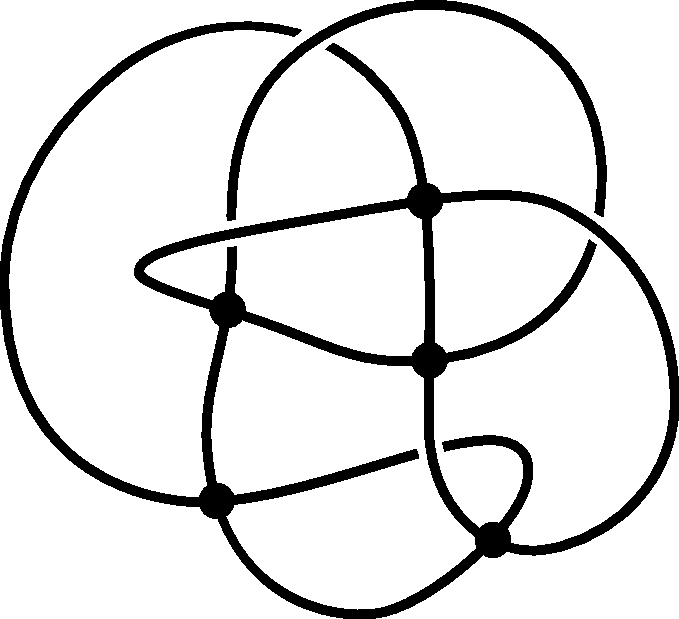
\includegraphics[width=0.14\textwidth, valign=c]{graphics/knot_9_33_singular.pdf}
		\quad \overset{\pi}{\longmapsto} \quad
		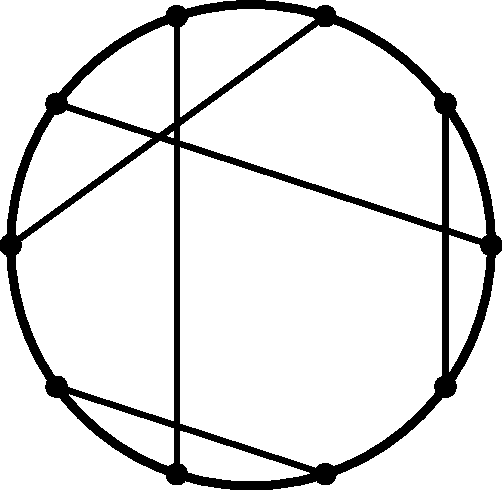
\includegraphics[width=0.13\textwidth, valign=c]{graphics/chord_diagram_of_knot_9_33_singular.pdf}
	\]
\end{example}

\begin{proposition}
	Suppose \(P\) is an integrable \(m\)-singular invariant with integral \(Q\). Let \(Q_{0}\) differ from \(Q\) by a function on chord diagrams, that is
	\[Q_{0}(k) = Q(k) + q(\pi(k))\]
	for \(q \in \mathcal{D}_{m}^{\ast}\)
	Then \(Q_{0}\) is also an integral of \(P\).
\end{proposition}

\begin{proof}
	The derivative of a function of chord diagrams is zero, as two knots which differ by a crossing change have the same chord diagram. Hence \(Q\) and \(Q_{0}\) have the same derivative: \(P\).
\end{proof}

\begin{remark}
	We defined a constant of integration as a set of objects (e.g. \(c \in \mathcal{D}_{m}\)) but perhaps it would have been more accurate to define it as a functional (e.g. \(q \in \mathcal{D}_{m}^{\ast}\)). After all the constant of integration on the real line is ``\(+ \ C\)'' rather than the set \(\{\ast\}\) with one object. There is no real risk of confusion, so let us be slightly loose and use the terminology for either.
\end{remark}

Since we are trying to integrate more than once, we might wish to know which constants of integration are themselves integrable.

\begin{definition}
	\label{def:weight-system}
	A \textbf{weight system} is an integrable \(w \in \mathcal{D}_{m}^{\ast}\).
\end{definition}

If we take the relations for a knot invariant to be integrable and project them into the space of chord diagrams, we get the following relations.

\begin{definition}
	\label{def:ft-ot-relations}
	\begin{enumerate}
		\item The \textbf{four-term relation} is the relation
			\begin{mdframed}
				\begin{equation}
					\label{eq:four-term}
					\tag{\ft}
					4T = 0
				\end{equation}
			\end{mdframed}

		\item The \textbf{one-term relation} is the relation
			\begin{mdframed}
				\begin{equation}
					\label{eq:one-term}
					\tag{\ot}
					1T = 0
				\end{equation}
			\end{mdframed}
	\end{enumerate}
\end{definition}

\begin{proposition}
	A weight system is characterised as a constant of integration that satisfies \textup{\ref{eq:four-term}} and \textup{\ref{eq:one-term}}.
\end{proposition}
\begin{proof}
	A weight system defines an \(m\)-singular invariant that is also invariant under crossing change. To integrate it must satisfy \ref{eq:four-term}  and \ref{eq:one-term}. Since crossing changes are free, this is equivalent to satisfying the projection of \ref{eq:topological-four-term} and \ref{eq:topological-one-term} into chord diagrams.
\end{proof}




We return now to the secondary (and higher) obstructions. A general integral of on \(m\)-singular \(P\) is of the form
\[Q + q \circ \pi.\]
Since integration is linear, to be integrable again, both terms need to be integrable. The latter we have just seen as the condition that \(q\) is a weight system. A sufficient condition for the former to be integrable is that \(S\mathcal{K}_{m}\) vanishes. But this is a tautological statement of the general theory --- it doesn't mean much when we don't know what \(S\mathcal{K}_{m}\) is.

\begin{conjecture}
	\label{conj:every-t4t-t1t-integrates}
	An invariant of \(m\)-singular knots satisfying \textup{\ref{eq:topological-four-term}} and \textup{\ref{eq:topological-one-term}} integrates \(m\) times into a genuine knot invariant.
\end{conjecture}

\begin{remarks}
	\begin{enumerate}
		\item At first glance, this conjecture looks like it follows from Theorem~\ref{thm:stanford-integrates-once}. The point is that it may not be possible to choose the integral to again satisfy \(\ref{eq:topological-four-term}\) and \(\ref{eq:topological-one-term}\), which is what \(S\mathcal{K}\) measures.
		\item Computing \(S\mathcal{K}_{m}\) is dual to computing \(\ker \partial_{m + 1} \partial_{m} / \ker \partial_{m}\) (we saw a similar thing with the primary obstructions). Computing \(\ker \partial^{2}\) is the hard part --- it's not too hard to find some elements, but whether they form a spanning set is open.
		% TODO: Expand this out into a little interlude on graph cohomology?
		\item This conjecture is proven in certain cases. It holds the integration theory for braids \cite{integration-of-singular-braid-invariants}. In a certain sense it's ``half''-proven for knots \cite{a-combinatorial-half-integration-from-weight-system-to-vassiliev-knot-invariant}. In Chapter \ref{ch:combinatorial-integration_of_weight_systems} we extend this to ``a little more than half''.
	\end{enumerate}
\end{remarks}

% NOTE: Finite type/Vassiliev invariants definiions and take duals and end up with chord diagram algebra.

\begin{theorem}[Fundamental theorem of Vassiliev invariants]
	\label{thm:fundamental-theorem-of-vassiliev-invariants}
	Let \(f\) be an invariant of \(m\)-singular knots satsifying \textup{\ref{eq:topological-four-term}}, \textup{\ref{eq:topological-one-term}} and the additional condition that \(\delta f = 0\). Then \(f\) integrates \(m\) times into a genuine knot invariant.
\end{theorem}

\begin{corollary}
	The fundamental theorem of Vassiliev invariants holds even if the additional condition is replaced by \(\delta^{k} f = 0\) for some \(k\).
\end{corollary}


% TODO: Reformulation of the Weierstrauss conjecture as the fact that no knot invariant extends to contradict the relations. Perhaps the chord diagram ncatlab statements about cohomology.


\section{Third subsection}
